\section{Fundamentals of Quantum Computation}%
\label{quantum-computation}

The fundamental idea permitting gate-based quantum computation to represrent exponentially scaling fermionic wavefunctions using polynomially scaling quantum resources is its ability to encode and manipulate superpositions of states. In this section, we will provide an introduction to qubits and basic quantum gates.

\subsection{Introduction to Qubits}

Classical computation encodes information using binary strings formed from the computational basis states 0 and 1. Thus, given $n$ classical bits, we can encode $2^n$ binary strings. In contrast, information on a quantum computer is encoded using quantum states corresponding to vectors in a two-dimensional complex Hilert space $\mathbb{C}$. The $Z$ eigenbasis $\ket 0$ and $\ket 1$ are the eigenstates of the Pauli $Z$ matrix, and form the computational basis for quantum computation.

\begin{figure}[H]
    \centering
    \begin{minipage}{.45\textwidth}
        \centering
        \includezxdiagramtext{chapter-1/zero}{0.35}{
        \begin{pmatrix} 1 \\ 0 \end{pmatrix}}
    \end{minipage}%
    \begin{minipage}{0.45\textwidth}
        \centering
        \includezxdiagramtext{chapter-1/one}{0.35}{
        \begin{pmatrix} 0 \\ 1 \end{pmatrix}}
    \end{minipage}
    \caption{Computational $Z$ basis states.}
    \label{z-eigenstates}
\end{figure}

An arbitrary qubit state $\ket\psi$ can be described as a complex linear combination of the computational basis states $\ket\psi = \alpha\ket 0 + \beta\ket 1$ provided that the qubit state is normalised, $|\alpha|^2 + |\beta|^2 = 1$. In other words we require two complex numbers ($\alpha$ and $\beta$), or four real numbers, to describe an arbitrary qubit state. Since only the relative phase between the basis states is directly measureable, there is a redundancy in this description that allows us to represent an arbitrary qubit state using only three real numbers.

By taking advantage of this redundancy, we can derive a three-dimensional representation of an arbitrary qubit state, known as the Bloch sphere. Note that opposite points on the Bloch sphere correspond to mutually orthonal states (see the $Z$ eigenbasis in Figure \ref{z-eigenstates}). We could have equivalently chosen any pair of orthonormal states to form the computational basis. For instance, we define the $X$ eigenstates as follows.

\begin{figure}[H]
    \centering
    \begin{minipage}{.45\textwidth}
        \centering
        \includezxdiagramtext{chapter-1/plus}{0.4}{
        \frac{\ket 0 + \ket 1}{\sqrt 2}}
    \end{minipage}%
    \begin{minipage}{0.45\textwidth}
        \centering
        \includezxdiagramtext{chapter-1/minus}{0.4}{
        \frac{\ket 0 - \ket 1}{\sqrt 2}}
    \end{minipage}
    \caption{Computational $X$ basis states.}
    \label{x-eigenstates}
\end{figure}

In theory, a qubit can exist in an infinite number of states, however, upon measuring the qubit state with respect to a particular basis, the qubit state collapses into one computational basis state or the other. This result is known more formally as the \textit{no-cloning theorem}, which states that we cannot create indentical and independent copies of an arbitrary qubit state, as this would involve first measuring that state.

\subsection{Multiple-Qubit States}

Let us now consider systems consisting of multiple qubits. Similarly to how $n$ classical bits give rise to $2^n$ binary strings, we have that $n$ qubits give rise to $2^n$ basis states. These basis states are formed by taking the Kronecker. For instance, a two-qubit system gives rise to the four following basis states.
\begin{equation*}
    \ket{00} = \ket 0 \otimes \ket 0 \qquad
    \ket{01} = \ket 0 \otimes \ket 1 \qquad
    \ket{10} = \ket 1 \otimes \ket 0 \qquad
    \ket{11} = \ket 1 \otimes \ket 1
\end{equation*}
An arbitrary $n$-qubit \textit{state vector}, describing the state of the entire system, can be formed by taking a complex linear combination of the $2^n$ basis states. Therefore, in order to fully describe an arbitrary $n$-qubit state vector, we need to specify $2^n$ complex coefficients. In the case of a two-qubit system, we have the following.
\begin{gather*}
    \ket\psi =
    \alpha \ket{00} +
    \beta \ket{01} +
    \gamma \ket{10} +
    \delta \ket{11} \\
    \text{where} \,\,\,\, \alpha, \, \beta, \, \gamma, \, \delta \in \mathbb{C}
\end{gather*}

\subsection{Introduction to Quantum Gates}%
\label{quantum-gates}

Quantum gates, by definition, correspond to unitary transformations, $U^{-1} = U^\dagger$ \cite{Nielsen2012}. In other words, any quantum gate corresponds to a square unitary matrix that conserves the complex inner product of the state it acts on. Consequently, quantum gates can be viewed as rotations of the qubit state vector in Hilbert space. Let us introduce the most fundamental gates in quantum computation, known as the Pauli gates. The Pauli gates are described by the Pauli matrices: $2 \times 2$ matrices that rotate an arbitrary qubit state by $\pi$ radians about their respective axes.

\begin{figure}[H]
    \centering
    \begin{equation*}
        I = \begin{pmatrix} 1 & 0 \\ 0 & 1\end{pmatrix} \qquad
        X = \begin{pmatrix} 0 & 1 \\ 1 & 0\end{pmatrix} \qquad
        Y = \begin{pmatrix} 0 & -i \\ i & \,\,\,\,0\end{pmatrix} \qquad
        Z = \begin{pmatrix} 1 & \,\,\,0 \\ 0 & -1\end{pmatrix}
    \end{equation*}
    \caption{The Pauli matrices corresponding to the Pauli gates.}
    \label{pauli-matrices}
\end{figure}

The Pauli $X$ gate is the quantum analogue of the classical NOT gate in that it maps $\ket 0 \leftrightarrow \ket 1$. Importantly, the Pauli $X$ differs from its classical counterpart in that it can act on any arbitrary qubit state. Similarly, we have that the Pauli $Z$ gate maps $\ket + \leftrightarrow \ket -$ and the Pauli $Y$ gate maps $\ket R \leftrightarrow \ket L$.

% \begin{figure}[H]
%     \centering
%     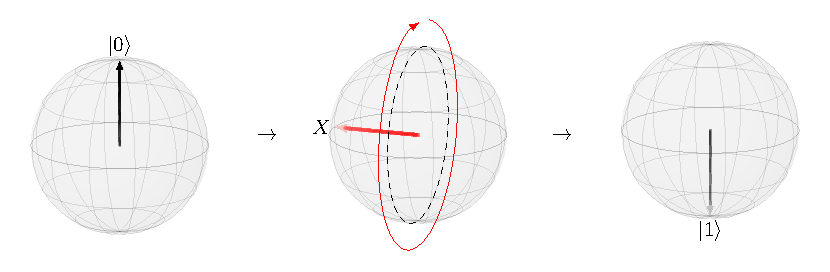
\includegraphics[width=0.6\linewidth]{chapter-1/zero_one}
%     \caption{Pauli $X$ gate acting on the $\ket 0$ state.}
% \end{figure}

% \begin{figure}[H]
%     \centering
%     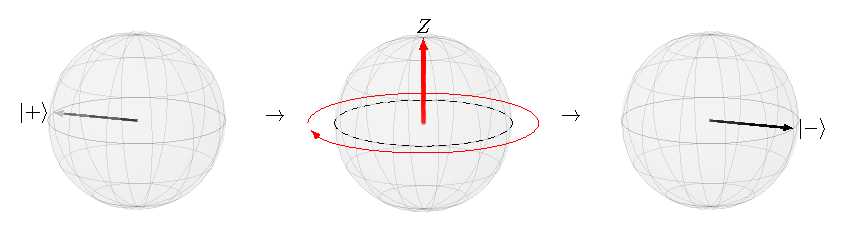
\includegraphics[width=0.6\linewidth]{chapter-1/plus_minus}
%     \caption{Pauli $Z$ gate acting on the $\ket +$ state.}
% \end{figure}

The Hadamard gate interconverts between the $Z$ and $X$ bases and maps $\ket 0 \leftrightarrow \ket +$ and $\ket 1 \leftrightarrow \ket -$. The Hadamard gate can, therefore, be viewed as a rotation of the Bloch sphere $\pi$ radians about the line bisecting the $z$ and $x$ axes.

\begin{figure}[H]
    \centering
    \includezxdiagramtext{chapter-1/hadamard}{0.15}{
    \frac{1}{\sqrt 2} \begin{pmatrix} 1 & 1 \\ 1 & -1 \end{pmatrix}}
    \caption{Bloch sphere represrentation of the Hadamard gate.}
\end{figure}

Since the Pauli gates and the Hadamard gate each correspond to unitary and Hermitian matrices, it follows that they are also self-inverse. Consequently, successively applying a Pauli or Hadamard twice is equivalent to applying the identity Pauli matrix, $I$, or applying no transformation at all.

The R$_Z(\theta)$ and R$_X(\theta)$ rotation gates correspond to rotations of the Bloch sphere by some angle $\theta$, in the $Z$ and $X$ bases respectively.

\begin{figure}[H]
    \centering
    \begin{minipage}{0.45\textwidth}
        \centering
        \includezxdiagramtext{chapter-1/z_rotation}{0.4}{
        \begin{pmatrix} 1 & 0 \\ 0 & e^{i\theta} \\ \end{pmatrix}}
    \end{minipage}
    \begin{minipage}{0.45\textwidth}
        \centering
        \includezxdiagramtext{chapter-1/x_rotation}{0.35}{
        \begin{pmatrix}
              1 + e^{i\theta} & 1 - e^{i\theta} \\
              1 - e^{i\theta} & 1 + e^{i\theta}
        \end{pmatrix}}
    \end{minipage}
    \caption{Bloch sphere representations of arbitrary $Z$ and $X$ rotations.}
\end{figure}

\subsection{Multiple-Qubit Gates}

The most fundamental multi-qubit gate is the two-qubit CNOT gate, which is used to entangle two qubits. Consider a two-qubit state of the form $\ket \alpha \otimes \ket \beta$. Taking $\alpha$ to be the control qubit and $\beta$ to be the target qubit, we define the CNOT gate as the gate that acts on the $\ket\alpha\otimes\ket\beta$ state to give the $\ket\alpha\otimes\ket{\alpha\oplus\beta}$ state. That is, the CNOT gate applies the Pauli $X$ gate to the target qubit \textit{iff} the control qubit is in the $\ket 1$ state. The CNOT gate acts on the two-qubit basis states as follows.
\begin{equation*}
    \ket{00} \rightarrow \ket {00} \qquad
    \ket{01} \rightarrow \ket {01} \qquad
    \ket{10} \rightarrow \ket {11} \qquad
    \ket{11} \rightarrow \ket {10}
\end{equation*}
In this way the CNOT gate is the quantum generalisation of the classical XOR gate. We define the two matrices corresponding to the CNOT gates (with the control and target qubits interchanged), as follows.

\begin{figure}[H]
    \centering
    \begin{equation*}
    \text{CNOT}^{c=0}_{t=1} =
        \begin{pmatrix}
            1 & 0 & 0 & 0 \\
            0 & 1 & 0 & 0 \\
            0 & 0 & 0 & 1 \\
            0 & 0 & 1 & 0
        \end{pmatrix} \qquad
        %
        \text{CNOT}^{c=1}_{t=0} =
        \begin{pmatrix}
            1 & 0 & 0 & 0 \\
            0 & 0 & 0 & 1 \\
            0 & 0 & 1 & 0 \\
            0 & 1 & 0 & 0
        \end{pmatrix}
    \end{equation*}
    \caption{Matrix definitions of the CNOT gates with the control and target qubits interchanged.}
\end{figure}

The CNOT gate can be used to entangle two qubits when the control qubit exists in a superposition of states. For instance, the CNOT gate acts on $\ket{+0}$ as follows.
\begin{equation*}
    \text{CNOT} \ket{+ \, 0} = \frac{\ket{00} + \ket{11}}{\sqrt 2}
\end{equation*}

% \subsection{Quantum Circuits}

% The research presented in this thesis revolves around the manipulation of \textit{quantum circuits} using a diagrammatic language known as the ZX calculus, which we introduce in more detail in Section \ref{zx-calculus}. Quantum circuits are composed of quantum gates (unitary transformations), such that the resulting quantum circuit itself, corresponds to a $2^n \times 2^n$ unitary transformation. This unitary transformation then acts on an $n$-qubit input vector to produce an $n$-qubit output vector. Below we summarise the representation of some of these quantum gates in the ZX calculus.

% \begin{figure}[H]
%     \centering
%     \begin{minipage}{0.45\textwidth}
%         \centering
%         \includezxdiagramtext{figures/chapter-2/pauli_z}{0.25}{
%         \begin{pmatrix} 1 & \,\,0 \\ 0 & -1 \end{pmatrix}}
%     \end{minipage}
%     \begin{minipage}{.45\textwidth}
%         \centering
%     \includezxdiagramtext{figures/chapter-2/pauli_x}{0.25}{
%     \begin{pmatrix} 0 & 1 \\ 1 & 0 \end{pmatrix}}
%     \end{minipage}%
%     \caption{Representation of the Pauli $Z$ and Pauli $X$ gates in the ZX calculus.}
% \end{figure}

% \begin{figure}[H]
%     \centering
%     \includezxdiagramtext{figures/chapter-1/hadamard_zx}{0.16}{
%     \frac{1}{\sqrt 2} \begin{pmatrix} 1 & 1 \\ 1 & -1 \end{pmatrix}}
%     \caption{Representation of the Hadamard gate in the ZX calculus.}
% \end{figure}


% \begin{figure}[H]
%     \centering
%     \begin{minipage}{0.45\textwidth}
%         \centering
%         \includezxdiagramtext{chapter-2/cnot}{0.25}{
%             \begin{pmatrix}
%             1 & 0 & 0 & 0 \\
%             0 & 1 & 0 & 0 \\
%             0 & 0 & 0 & 1 \\
%             0 & 0 & 1 & 0
%             \end{pmatrix}
%         }
%     \end{minipage}
%     \begin{minipage}{.45\textwidth}
%         \centering
%         \includezxdiagramtext{chapter-2/cnot2}{0.25}{
%         \begin{pmatrix}
%         1 & 0 & 0 & 0 \\
%         0 & 0 & 0 & 1 \\
%         0 & 0 & 1 & 0 \\
%         0 & 1 & 0 & 0 \\
%         \end{pmatrix}}
%     \end{minipage}%
%     \caption{Representation of the CNOT gates in the ZX calculus, with the control and target qubits interchanged.}
% \end{figure}

